% =====================================================================
%  chunks/ch04k.tex —— 原书 p.259–272（PDF 266–279）
%  第 4 章 §5（下）：非单连通流形分类、高阶符号差、Hermitian K 理论、
%  几何拓扑、Milnor 例子、环带猜想、拓扑与 PL 结构
% =====================================================================
% [原文 p.259]
\[
B(\eta)\colon
\begin{cases}
\eta_{n}\mapsto\eta_{n+1},\\
\bar\eta_{n}\mapsto\bar\eta_{n}.
\end{cases}
\tag{5.13}
\]
$\bar B$ 的定义如下：秩为 $N$ 的自由 $A[t,t^{-1}]$-模 $F_{N}$ 的每个自同构 $\lambda$，在乘以 $t$ 的足够大的幂 $n$ 之后，都可相对于 $F_{N}$ 的某个基 $e_{1},\dots,e_{N}$ 用 $A[t]$ 上的矩阵表示。把 $F_{N}$ 的「正部分」记作
\[
F_{N}^{+}=\Bigl\{\sum a_{j}e_{j}\ \Big|\ a_{j}\in A[t]\Bigr\},
\]
我们令
\begin{equation}
\bar B(\lambda)=F_{N}^{+}/t^{n}\lambda=\eta. \tag{5.14}
\end{equation}
容易验证模 $\eta$ 的投射性，从而验证 $\bar BB=1$ 在 $K_{0}(A)$ 上成立。

由此推出，恒有
\begin{equation}
K_{1}(A[t,t^{-1}])\cong K_{0}(A)\oplus K_{1}(A)\oplus P. \tag{5.15}
\end{equation}
在 $A=\Z[\pi]$、$\pi$ 为自由阿贝尔群的情形，Bass 证明了 $P=0$。由于对这种 $\pi$（$\cong\Z\oplus\dots\oplus\Z$），每个有限生成 $\Z[\pi]$-模都有长度有限的自由零调分解，且 $K_{0}(\pi)=0$，通过归纳便得到 Bass 关于自由阿贝尔 $\pi$ 的定理：
\[
Wh(\pi)=K_{1}(\pi)/\pm\pi=0.
\]
由此推出：在基本群为自由阿贝尔群的情形，上面提到的非单连通流形的不变量是平凡的。% [Tutor Note: 这里的 $P$ 是 $\tilde K_{0}$ 型的「Nil 项」；Bass 定理说自由阿贝尔群的 Whitehead 群消没，因此单纯从 $K$ 理论看不出非平凡性。若 $\pi$ 含挠或非交换，$Wh(\pi)$ 一般非零，这正是 $h$-配边障碍的来源。]

这类问题的一个自然延续是：把流形 $W^{n}$ 表示为圆周上的光滑纤维丛（$W^{n}\to S^{1}$），并假定给定的流形 $W^{n}$ 具有这样的丛的同伦型。若 $\pi_{1}(W^{n})\cong\Z$、$n\ge 6$，且纤维化（fibration）的纤维单连通，则该问题有肯定的解答（Browder、Levine、Livesay，1960 年代中期）。在更一般的情形，即纤维非单连通时，出现的障碍同时涉及 $K_{0}(\pi)$ 与 $K_{1}(\pi)$，其中 $\pi$ 是纤维的基本群，即同态 $f_{*}\colon\pi\to\Z$ 的核 $\operatorname{Ker}f_{*}$，而该同态由适当选取的映射 $f\colon W^{n}\to S^{1}$（作为光滑投影的候选者）诱导。（这一问题的解决在 1960 年代后半期由 Hsiang 与 Farrell 得到。）

现在转向维数 $n\ge 5$ 的非单连通流形的一般分类理论。这一理论紧承 Browder--Novikov 关于分类维数 $n\ge 5$ 的单连通流形的方案（见上文 §4）；然而它并不给出最终分类定理，而是把问题归结为某些代数障碍的存在性，下面就来描述这些障碍。Browder--Novikov 装置的全部（已在 §4 中描述），包括闭流形的 1 次正规映射（normal map）以及它们之间的配边，都可以搬到非单连通情形。
% [原文 p.260]
利用 Hurewicz 定理的非单连通类比（它涉及 1 次正规映射 $f\colon M_{1}\to M$ 所诱导同态的核），可以对这样的映射作 Morse 手术，把它变成使相应的同伦群直到维数 $[n/2]-1$（含）都同构的映射。对偶数 $n$（$=2k$），对第 $k$ 维同伦核的分析（借助万有覆叠流形）表明：该核是有限生成的自由稳定 $\Z[\pi]$-模，其上定义有由提升到万有覆叠流形上的闭链的相交指数给出的 $\pi$-不变标量积：
\begin{equation}
\langle z,w\rangle=\sum_{\sigma\in\pi}(z\circ\sigma w)\in\Z[\pi]. \tag{5.16}
\end{equation}
于是这个标量积取值于 $\Z[\pi]$，而 $\Z[\pi]$ 上有对合 $u\mapsto\bar u$，其中
\begin{equation}
u=\sum_{i}a_{i}g_{i},\quad a_{i}\in\Z,\quad g_{i}\in\pi,\qquad
\bar u=\sum_{i}a_{i}g_{i}^{-1}, \tag{5.17}
\end{equation}
它具有对合的通常性质：
\begin{equation}
\overline{uv}=\bar v\bar u,\qquad \bar{\bar u}=u. \tag{5.18}
\end{equation}

\begin{remark}
注意，对不可定向流形，对合的定义须作如下调整：
\begin{equation}
u\mapsto\bar u=\sum_{i}(\sgn g_{i})a_{i}g_{i}^{-1}, \tag{5.19}
\end{equation}
其中当 $g_{i}$ 的作用反转定向时 $\sgn g_{i}=-1$，否则 $\sgn g_{i}=+1$。\hfill$\square$
\end{remark}

标量积 (5.16) 在 $k$ 为偶数时是 Hermitian 的，在 $k$ 为奇数时是余 Hermitian 的：
\begin{equation}
\begin{gathered}
\langle uz,w\rangle=u\langle z,w\rangle,\qquad \langle z,w\rangle=\pm\langle w,z\rangle,\\
\langle z,uw\rangle=\langle z,w\rangle\bar u,
\end{gathered} \tag{5.20}
\end{equation}
并且是非退化的，其含义是：相对于 $\Z[\pi]$-模 $M=\operatorname{Ker}f_{*}^{(\pi_{k})}$（$n=2k$）的自由基底 $\{e_{i}\}$，矩阵
\[
B=(b_{ij})=(\langle e_{i},e_{j}\rangle)
\]
可逆。（回忆一下，我们已经处在 $\operatorname{Ker}f_{*}^{(\pi_{j})}=0$（$j<k$）的情形。）用不变的形式（即不参照任何基来表达）说，这种非退化性意味着标量积 $\langle\ ,\ \rangle$ 决定一个同构
% [原文 p.261]
\[
h\colon\mathcal M\to\mathcal M^{*}=\operatorname{Hom}_{A}(\mathcal M,A),\qquad A=\Z[\pi],
\]
它由
\begin{equation}
u\mapsto h(u),\qquad \langle h(u),v\rangle=\langle u,v\rangle \tag{5.21}
\end{equation}
给出。（注意，上述对合使得 $\mathcal M^{*}$ 可以具有 $\Z[\pi]$-模的结构。）这个标量积具有「偶性」，用矩阵的语言说（在模 $\mathcal M$ 自由的情形下），这意味着上述矩阵 $B$ 可表为
\[
B=V\oplus(-1)^{k}V^{+},
\]
其中 $V^{+}=\bar V^{T}$，$T$ 表示转置运算。对奇数 $k$，还存在 $\Z/2$-不变量（类似于 Arf 不变量），不过我们不在此描述。若 $M^{n}$ 既不是光滑流形也不是 PL 流形，而只是 $\Z[\pi]$-同调与上同调满足 Poincaré 对偶的 CW 复形，则模 $\mathcal M=\operatorname{Ker}f_{*}^{(\pi_{k})}$ 将只是投射 $\Z[\pi]$-模，而不是稳定自由的。此时可以几何地行事：通过粘上指数为 $k$ 的把手来增加生成元，以便把投射模 $\mathcal M$ 变成稳定自由模。这时障碍出现在 Hermitian 群与余 Hermitian 群 $K_{0}^{h}(\Z[\pi])$、$K_{0}^{sh}(\Z[\pi])$ 中，与前面一样。在此框架下，平凡元素的角色由这样一个模（记作 $H_{g}$）担任：它具有典范的闭链基，这些闭链相对于标量积的行为，类似于亏格 $g$ 曲面上标准闭链相对于相交指数的行为：
\begin{equation}
\begin{gathered}
a_{1},\dots,a_{g},\qquad b_{1},\dots,b_{g},\\
\langle a_{i},a_{j}\rangle=0,\quad \langle b_{i},b_{j}\rangle=0,\quad
\langle a_{i},b_{j}\rangle=\delta_{ij}=\pm\langle b_{j},a_{i}\rangle.
\end{gathered} \tag{5.22}
\end{equation}
在取模的直和这一运算下，并对所有 $g$ 施加关系 $H_{g}\sim 0$，便得到 Grothendieck 群的如下类比：
\[
\begin{gathered}
K_{0}^{h}(\Z[\pi])\quad(k\ \text{为偶数，Hermitian 情形}),\\
K_{0}^{sh}(\Z[\pi])\quad(k\ \text{为奇数，余 Hermitian 情形}),
\end{gathered}
\]
其中 $\Z[\pi]$ 带有对合 (5.17)（在不可定向情形下则是 (5.19)）。

Morse 手术的障碍理论的代数表述，在 $n=2k$ 的情形由 Novikov 与 Wall 在 1960 年代中期给出，并由 Wall 在 1960 年代末推广到奇数 $n$。结果表明，障碍归结为群 $K_{1}^{h}(\Z[\pi])$（$k$ 为偶数）与 $K_{1}^{sh}(\Z[\pi])$（$k$ 为奇数）的元素；这两个群仿照群 $K_{1}(\pi)$ 构造，所用的是由 (5.22) 定义、保持标量积的典范模的自同构的稳定类。
% [原文 p.262]
在这些类上施加 Whitehead 关系（即把这些自同构的直和与它们对应的复合视为等同），即得到交换性；此外还须再加一个关系，后者可方便地表述为：任何满足 $\lambda(a_{j})=a_{j}$（$j=1,\dots,g$）的自同构 $\lambda\colon H_{g}\to H_{g}$ 都令其等于平凡自同构。这些由环 $\Z[\pi]$ 上自由模的自同构定义的手术障碍群，称为 $\pi$ 的\emph{Wall 群}，记作 $L_{n}(\pi)$：
\begin{equation}
L_{0}\cong K_{0}^{h},\qquad L_{1}\cong K_{1}^{h},\qquad
L_{2}\cong K_{0}^{sh},\qquad L_{3}\cong K_{1}^{sh}. \tag{5.23}
\end{equation}
如前所述，我们不在此讨论这些群的 $\Z/2$-结构以及与之相伴的 Arf 不变量的类比。

还有另一种途径（沿着上一段之前所描述的思路）来定义群 $K_{0}^{h}$、$K_{1}^{h}$、$K_{0}^{sh}$、$K_{1}^{sh}$：用带非退化 Hermitian 或余 Hermitian 标量积（并具有所需的「偶性」以及 Arf 不变量所承载的结构）、决定同构 $h\colon\mathcal M\xrightarrow{\ \cong\ }\mathcal M^{*}$、且取值于带对合的环中的投射模来定义。（在上面的拓扑背景中，该环是 $\Z[\pi]$，对合 $u\to\bar u$ 如 (5.17) 或 (5.19) 所述。）群 $\tilde K_{0}^{h}$ 与 $\tilde K_{0}^{sh}$ 按通常方式用这类模的直和来定义，并施加把形如 $M=N\oplus N^{*}$（$N^{\ast\ast}\cong N$）的投射模等同于平凡模的关系：
\begin{equation}
\begin{gathered}
\langle N,N\rangle=\langle N^{*},N^{*}\rangle=0,\\
N\oplus N^{*}\sim 0,\qquad h\colon N\oplus N^{*}\to(N\oplus N^{*})^{*},
\end{gathered} \tag{5.24}
\end{equation}
其中同构 $h$ 由一对典范同构给出：
\begin{equation}
h\colon
\begin{cases}
N^{*}\xrightarrow{\ \cong\ }N^{*},\\
N\xrightarrow{\ \cong\ }N^{\ast\ast}.
\end{cases} \tag{5.25}
\end{equation}
$\tilde K_{1}^{h}$ 与 $\tilde K_{1}^{sh}$ 的代数定义不基于自同构（如上），而基于如下概念：典范投射模 $N\oplus N^{*}$ 的\emph{Lagrange 子模} $L\subset N\oplus N^{*}$，它由条件 $h|_{L}=0$ 以及 $L$ 是满足
\begin{equation}
M=N\oplus N^{*}\sim L\oplus L^{*},\qquad L^{\ast\ast}=L \tag{5.26}
\end{equation}
的直和项来定义。群运算由对 $(M,L)$ 的直和给出；那些使投影 $M\to N$（$N^{*}\to 0$）限制为同构 $L\to N$ 的对 $(M,L)$ 取为平凡。而 $(M,L)$ 的稳定等价类构成群 $\tilde K_{1}^{h}$ 与 $\tilde K_{1}^{sh}$，即 Novikov--Wall 群。

不考虑可能的变体、也不深入细节，我们指出：对任何带对合 $u\to\bar u$（$\bar u\bar v=\overline{vu}$）的环 $A$，在自由情形与投射情形下都可以定义高阶类比 $\tilde K_{i}^{h}$ 与 $\tilde K_{i}^{sh}$。结果表明，例如 $\tilde K_{2}^{h}=K_{0}^{sh}$，而 $K_{2}^{sh}=K_{0}^{h}$。% [Tutor Note: 这一段把手术障碍翻译成纯代数：Wall 群 $L_{n}(\pi)$ 与 Hermitian $K$ 群 $\tilde K_{i}^{h,sh}$ 只差指标平移（$L_{0}\cong K_{0}^{h}$ 等）。记忆要点是「偶／余偶」随维数奇偶而互换，这正是 (5.23) 中下标交替的原因。]
% [原文 p.263]
群 $K_{i}^{h}\otimes\Z[\tfrac12]$、$K_{i}^{sh}\otimes\Z[\tfrac12]$ 的一个代数理论，由 Novikov（1960 年代末）在带对合的环的范畴中表述出来，其中包含 Bass 投影算子（见上）之类比物的代数构造：
\begin{equation}
K_{i}^{h}(A[t,t^{-1}])\ \underset{\bar B}{\overset{B}{\rightleftarrows}}\ K_{i+1}^{h}(A),\qquad \bar BB=1. \tag{5.27}
\end{equation}
群 $K_{i}^{h}\otimes\Z[\tfrac12]$ 在带对合的环的范畴中给出一个周期的（周期 4 的）同调理论；在其中，Bass 投影算子 (5.27) 的 Hermitian 类比物由于同构
\begin{equation}
K_{j}^{h}\cong K_{j+2}^{sh},\qquad K_{j}^{sh}\cong K_{j+2}^{h} \tag{5.28}
\end{equation}
而把余 Hermitian 情形也涵盖进来。在这方面请注意同构（模去与 $\Z[\tfrac12]$ 作张量积）
\begin{equation}
K_{j+1}^{h}(A[t,t^{-1}])\cong K_{j}^{h}(A)\oplus K_{j+1}^{h}(A), \tag{5.29}
\end{equation}
它与通常 $K$-理论中相应的情形（那里有非平凡的核 $N$）形成对照。

上述 Hermitian $K$ 理论（按 Novikov 的表述方式）利用了对上述代数对象的几何实现的分析，以及在与分析和量子力学相联系中出现的 Hamilton 形式体系诸概念的类比物；这些类比物在 1960 年代初被 Maslov 密集地用于双曲型方程理论中短波渐近展开的构造（并由许多作者进一步发展）。一旦翻译到代数背景中，辛几何与 Hamilton 形式体系的标准术语就变得极为有用；特别地，它澄清了代数构造背后的想法（有时甚至提示了恰当的想法），并使 Bott 周期性的代数类比物背后的机制更加明显。当然，代数理论一旦被精确表述，就不再依赖于它与 Hamilton 形式体系的类比这一来源。

Mishchenko 证明（约 1970 年），与 $\Z[\tfrac12]$ 作张量积可以消除各种已提出的 Hermitian $K$ 理论之间的差别。与此同时，他构造了可定向流形 $M^{j}$ 的一个同伦不变量 $\tau^{\pi}$，它由 $K_{j}^{h}(\Z[\pi])$（其中 $\pi=\pi_{1}M^{j}$）的一个元素给出，类似于符号差，并决定从 Eilenberg--MacLane 空间 $K(\pi,1)$ 的每个配边群到相应的 Hermitian $K$ 理论的同态：
\[
\tau^{\pi}\colon\Omega_{j}^{SO}(K(\pi,1))\to K_{j}^{h}(\Z[\pi])\otimes\Z[\tfrac12].
\]
对 1 次正规映射 $f\colon M_{1}^{n}\to M^{n}$（它在维数 $\ge 5$ 的流形的一般分类理论中居于中心地位），障碍由如下公式给出：
% [原文 p.264]
\[
\tau^{\pi}(M_{1}^{n})-\tau^{\pi}(M^{n})\in K_{n}^{h}(\Z[\pi])\otimes\Z[\tfrac12].
\]

\begin{remark}
注意，即使对单连通流形，若不除以 2，这类障碍的计算也是不可能的，其困难与 Arf 不变量有关。\hfill$\square$
\end{remark}

Novikov 的高阶符号差猜想，涉及 Chern 特征的一个纯代数类比物的存在性：
\[
\ch\colon K_{*}^{h}(\Z[\pi])\otimes\Q\to H_{*}(\pi;\Q),
\]
其性质是：对闭流形 $M^{n}$，下述公式应当成立：
\begin{equation}
\langle z,\ch\circ\tau^{\pi}(M^{n})\rangle=\langle L_{k}(M^{n}),D\phi^{*}(z)\rangle. \tag{5.30}
\end{equation}
这里 $\pi=\pi_{1}(M^{n})$，$\phi\colon M^{n}\to K(\pi,1)$ 是典范映射，$D\phi^{*}(z)\in H_{4k}(M^{n};\Q)$，$L_{k}$ 是 $M^{n}$ 的 Pontryagin 类中的 Hirzebruch 多项式。看来，这个公式若对任何群 $\pi$ 都成立，就将囊括流形 $M^{n}$ 在给定同伦型下 Pontryagin 类之间的一切可能关系。在一般高阶符号差猜想已被确立的一切情形中，这样的 Chern 特征代数类比物（满足 (5.30) 者）的存在性也都已被证明。

1960 年代后半期，I. M. Gel'fand 与 Mishchenko 注意到：对紧空间 $X$ 上复值函数的环 $C^{*}(X)$，有
\[
K_{0}^{h}(C^{*}(X))\cong K_{\C}^{0}(X).
\]
事实上，对 $K_{1}$ 也存在这样的同构，从而对这类带对合的函数代数的所有 $K_{*}^{h}$ 都存在（$C^{*}(X)$ 上的对合由 $f\to\bar f$ 给出）。在 $X=T^{n}$ 的情形，利用 Fourier 变换得到如下同构（模去与 $\Z[\tfrac12]$ 作张量积）：
\begin{equation}
K_{*}^{h}(\C[\Z\times\dots\times\Z])\cong K_{*}^{h}(C^{*}(T^{n}))
\quad(\cong K_{\C}^{*}(T^{n})). \tag{5.31}
\end{equation}
因此，$T^{n}$ 上向量丛的通常 Chern 特征，为 $\pi=\Z\times\dots\times\Z$（$n$ 个因子）提供了 Chern 特征的代数类比物；不过这种获得类比物的方法显然不是代数的。

对环 $C^{*}(X)$，$K_{*}^{h}$ 理论中 Bass 投影算子类比物的代数定义，给出一个悬挂同构，以及一条不同于 Atiyah 等人的通常 $K$-理论所提供的通向 Bott 周期性的途径。注意，环 $C^{*}(X)$ 中虚数 $i$（$i^{2}=-1$）的存在使得 Hermitian 理论可以转换为余 Hermitian 理论；于是对带有这种虚数元素的代数 $A$，有 $K_{*}^{h}(A)=K_{*}^{sh}(A)$，而周期性缩短为 2。

把各种代数构造梳理清楚之后，就可以从 Hamilton 形式体系的观点理解周期性的意义。
% [原文 p.265]
不过，这一理论（按 Novikov 在 1960 年代末的构想）涉及张量积 $K_{*}^{h}\otimes\Z[\tfrac12]$。Hermitian 代数 $K$ 理论（称为\emph{代数 $L$ 理论}）的完全形式化，不借助与 $\Z[\tfrac12]$ 作张量积，由 Ranicki 在 1970 年代前半期实现：他把理论重新建立在整数上；对群环 $\Z[\pi]$，相应的群记作 $L_{n}(\pi)$。这些群在整个 1970 年代直至 1980 年代为若干人所研究（Pedersen、Beck、Sharpe）。1970 年代前半期，Wall 与 Beck 对 $\pi$ 有限且模自由的情形发展了计算这些对象的细致技巧，并实际对各种具体的群完成了计算。

另一方面，尽管完整的代数理论直到 1960 年代末才具备，但更早就有可能在某些特殊情形（虽然是非有效的方式）得到群 $L_{n}(\pi)$ 的完整信息，而无须掌握代数定义的细节；例如当 $\pi$ 为自由阿贝尔群 $\pi=\Z\times\dots\times\Z$ 时。在 $\pi=\Z$ 的情形，这一理论由 Browder（1960 年代中期）表述为可化归到单连通情形的几何障碍理论。在这一形式下，理论随后由 Shaneson（1960 年代末）推广到更一般的 $\pi=\Z\times\dots\times\Z$。独立于群 $L_{n}(\pi)$ 的各种代数定义，存在同构
\begin{equation}
L_{n}(\pi\times\Z)\cong L_{n}(\pi)\oplus L_{n+1}(\pi), \tag{5.32}
\end{equation}
它可以用几何方式建立；这一同构使得群 $L_{n}(\Z\times\dots\times\Z)$ 的结构可以从群 $L_{n}(1)=L_{n}$ 的结构（非有效地）推断出来，后者如下：
\[
L_{n}\cong
\begin{cases}
\Z, & n\equiv 0\ (\mathrm{mod}\ 4),\\
\Z/2, & n\equiv 2\ (\mathrm{mod}\ 4),\\
0, & \text{其他情形}.
\end{cases}
\]
（这些同构早已由单连通手术理论得知。）知道群 $L_{n}(\Z\times\dots\times\Z)$ 之后，就可以得到同伦 $n$-环面的完全分类，即具有环面 $T^{n}$（$n\ge 5$）的同伦型的 $n$ 维流形的完全分类。特别地，结果表明：这样的流形总有一个与标准环面 $T^{n}$ 微分同胚的有限叶覆叠流形。

\begin{remark}
我们指出，所有手术障碍（即群 $L_{n+1}(\pi)$ 的元素）都几何地实现为区分给定 $n$ 维流形的同一同伦类中两个流形的不变量。构造如下：若两个正规映射 $f_{i}\colon M_{i}^{n}\to M^{n}$ 都是同伦等价且属于同一个正规配边类，则存在一个配边 $W^{n+1}$，其边界是 $M_{1}^{n}$ 与 $M_{2}^{n}$ 的不交并（$\partial W^{n+1}=M_{1}^{n}\sqcup M_{2}^{n}$），并连同正规映射 $F\colon W^{n+1}\to M^{n}\times I$，它在边界分支 $M_{1}^{n}$、$M_{2}^{n}$ 上的限制分别是 $f_{1}$、$f_{2}$。把 $p\colon M\times I\to M$ 记作到第一个因子的投影。

% [原文 p.266]
在上述条件下，映射 $F_{1}=f_{1}^{-1}\circ p\circ F$ 给出到边界分支 $M_{1}^{n}$ 上的正规收缩 $W^{n+1}\to M_{1}^{n}$（参看上文 §4）。从给定的流形 $M_{1}^{n}$ 出发，借助这样的配边 $W^{n+1}$，可以几何地实现手术障碍群的每个元素，正如在单连通情形一样。于是，可以从 $M_{1}^{n}$ 出发，构造与群 $L_{n+1}(\pi)\cong K_{n+1}^{h}(\pi)$ 中任给元素相对应的这样的配边 $W^{n+1}$。\hfill$\square$
\end{remark}

对同伦环面，存在一个指数有限的子群
\[
A_{n}\subset L_{n+1}(\Z\times\dots\times\Z),
\]
其元素由边界分支微分同胚（$M_{1}^{n}\cong M_{2}^{n}$，$\partial W^{n+1}=M_{1}^{n}\sqcup M_{2}^{n}$）的配边流形 $W_{n+1}$ 实现。这一定理（借助 Novikov 关于所有同伦环面都稳定平行化的结果）推出：每个正规配边类中不同同伦环面的个数有限（Wall、Siebenmann、Hsiang、Shaneson、Casson，1960 年代末）。

由于按 Shaneson 的一个定理，群
\[
L_{n+1}(\Z\times\dots\times\Z)\cong K_{n+1}^{h}(\Z\times\dots\times\Z)
\]
（模去一个有限群）由高阶符号差决定，所以关于每个正规配边类中同伦环面个数有限的结果，也可以由高阶符号差的 Hirzebruch 公式的非单连通类比推出；这与 Milnor 关于群 $bP^{4k}$ 有限性的定理由通常 Hirzebruch 公式推出大致是同样的方式。这里的论证如下。考虑环面 $T^{n+1}$ 上满足 $J(\xi_{N})=0$ 且 $\xi_{T^{n}}=0$ 的向量丛 $\xi_{N}$ 构成的群（即 $\xi_{N}$ 是环面 $T^{n+1}$ 上稳定同伦平凡的丛，而它到 $n$ 维环面 $T^{n}\subset T^{n+1}$ 的限制 $\xi_{T^{n}}$ 是平凡向量丛）。按正规配边的一般构造（参看上文 §4），得到一个映射
\[
S^{N+n+1}\to T\xi_{N},
\]
以及一个 1 次正规映射
\[
f\colon M^{n+1}\to T^{n+1},\qquad f^{*}(\xi_{N})\cong\nu_{M},
\]
其中 $M^{n+1}$ 是实现群
\[
L_{n}(\pi)\subset L_{n}(\pi\times\Z),\qquad
\pi=\underbrace{\Z\times\dots\times\Z}_{n\ \text{次}}
\]
的某个元素 $\alpha$ 的光滑闭流形；该元素由 Chern 特征 $D\ch\xi_{N}\in H_{*}(T^{n+1};\Q)$ 唯一确定（模 $2^{n}$）。于是上述构造给出一个 1 次正规映射：
\begin{center}
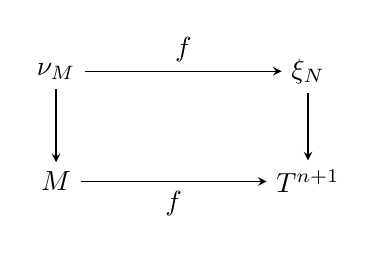
\begin{tikzpicture}[>=stealth,baseline=(current bounding box.center)]
  \node (a) at (0,1.4) {$\nu_{M}$};
  \node (b) at (3.2,1.4) {$\xi_{N}$};
  \node (c) at (0,0) {$M$};
  \node (d) at (3.2,0) {$T^{n+1}$};
  \draw[->] (a)--node[above]{$f$}(b);
  \draw[->] (c)--node[below]{$f$}(d);
  \draw[->] (a)--(c);
  \draw[->] (b)--(d);
\end{tikzpicture}
\end{center}

% [原文 p.267]
它在 $T^{n}\subset T^{n+1}$ 上是平凡的：
\[
f^{-1}(T^{n})\cong T^{n}\subset M^{n+1},\qquad
\nu_{M}|_{T^{n}}=f^{*}\xi_{N}|_{T^{n}}=0.
\]
然后沿嵌入的环面 $T^{n}$ 剪开 $M^{n+1}$，就得到实现元素 $\alpha$ 的所需流形，它的两个边界分支都微分同胚于 $T^{n}$。

给定两个 CW 复形或流形，人们常常借助代数拓扑不变量把它们区分开，即证明它们不同胚（或非 PL 同胚，或非微分同胚）。然而，若这两个空间的一切能设想的不变量都相同，那就不得不最终设法真正构造出它们之间的同胚。考察过去二三十年间为此目的而采用的各种方法，是很有意思的。在微分拓扑中，解决这一问题所依靠的，或者是直接用分析方法造出适当的映射，或者是使用完全有限性的程序，即仔细选取并分析把手的粘接序列（例如借助 Morse 手术，此时 Morse 函数的水平集的拓扑在其值经过临界点时发生变化）。在施行 Morse 手术序列时，人们会研究它们对同伦的影响、实现它们所出现的代数障碍，以及发生的各种约化和简化（例如一对把手的相互消去）。这些基本技巧已经使用了很长时间，在 1960 年代随着当时流形拓扑的卓越发展而得到密集的精细化。不过我们不在此进一步讨论它们；本书前面各处已经提到过。拓扑学还有哪些工具适合直接研究同胚？在低维（$n\le 3$），流形的每个紧族同胚都可用 PL 同胚逼近，也可用微分同胚逼近，并且流形的整个自同胚群的局部与整体同伦性质，与 PL 同胚群相同（Moise，1950 年代初），甚至与自微分同胚群也相同。然而在更高维，情况肯定不再如此。与这类问题有关的早期结果中，用初等视觉手段得到的最著名者之一，是 Mazur 与 Brown 的结果（约 1960 年）：
\begin{theorem*}{}
给定球面的一个「平坦」嵌入，即整个邻域的嵌入
\[
F\colon S^{n-1}\times I\to S^{n},\qquad I=[-1,1],
\]
则「中间」球面 $S^{n-1}\times\{0\}$ 的像 $F(S^{n-1}\times\{0\})$ 是闭圆盘 $D^{n}\subset S^{n}$ 的边界：$\partial D^{n}=F(S^{n-1}\times\{0\})$。
\end{theorem*}
（这就是「广义 Schoenflies 猜想」。）紧接 Brown--Mazur 定理出现之后，「环带猜想」被（若干人）提了出来：

% [原文 p.268]
给定 $S^{n}$ 中两个不相交的平坦嵌入 $F_{1}$ 与 $F_{2}$（$S^{n-1}\hookrightarrow S^{n}$）：
\[
F_{1}(S^{n-1}\times\{0\})\cap F_{2}(S^{n-1}\times\{0\})=\varnothing,
\]
它们之间 $S^{n}$ 的闭区域是否同胚于环带 $S^{n-1}\times I$？

对 $n\le 3$，这一猜想因初等理由成立；对 $n\ge 6$，在光滑性假设下由 Smale 的 $h$-配边定理成立。事实上，在更高维，只要嵌入 $F_{1}$、$F_{2}$ 至少在一点处光滑，环带猜想就不难建立。（下文我们还要回到环带猜想的讨论。）

现在描述 Mazur 的另一个结果（1960 年代初）：它虽然涉及光滑流形，却使用完全初等的技巧，并且可以证明某两个已知在组合上不等价的 CW 复形却仍然同胚（Milnor，也在 1960 年代初）。该定理如下：
\begin{theorem*}{}
若 $f\colon M_{1}^{n}\to M_{2}^{n}$ 是两个流形 $M_{1}^{n}$ 与 $M_{2}^{n}$ 之间的正规同伦等价，即 $f^{*}(\nu^{(2)})=\nu^{(1)}$，其中 $\nu^{(i)}$ 表示 $M_{i}^{n}$ 相对于嵌入 $M_{i}^{n}\subset\R^{N+n}$（$N\ge n+1$）的法丛，则直积
\[
M_{1}^{n}\times\R^{N}\quad\text{与}\quad M_{2}^{n}\times\R^{N}
\]
微分同胚。
\end{theorem*}

证明的想法如下：考虑嵌入
\begin{equation}
M_{1}^{n}\times D^{N}\hookrightarrow M_{2}^{n}\times\R^{N}
\quad\text{与}\quad
M_{2}^{n}\times D^{N}\hookrightarrow M_{1}^{n}\times\R^{N} \tag{5.33}
\end{equation}
它们分别「逼近」同伦等价 $f\colon M_{1}^{n}\to M_{2}^{n}$ 与同伦逆 $g\colon M_{2}^{n}\to M_{1}^{n}$（$f\circ g\sim 1$，$g\circ f\sim 1$）。$M_{2}^{n}\subset M_{1}^{n}\times\R^{N}$ 与 $M_{1}^{n}\subset M_{2}^{n}\times\R^{N}$ 的法丛（其中的包含映射是把上述嵌入限制到 $M_{1}^{n}\times\{0\}$ 与 $M_{2}^{n}\times\{0\}$ 得到的）由于假设 $f^{*}(\nu^{(2)})=\nu^{(1)}$ 而是平凡的。由这对嵌入 (5.33)，我们得到一个扩张的区域序列
\[
M_{1}^{n}\times D_{1}^{N}\subset M_{2}^{n}\times D_{2}^{N}
\subset M_{1}^{n}\times D_{3}^{N}\subset\cdots,
\]
其中球 $D_{i}^{N}\subset\R^{N}$ 的半径递增，所有嵌入
\[
M_{1}^{n}\times D_{2i+1}^{N}\hookrightarrow M_{1}^{n}\times\R^{N}
\]
都是标准的，而 $M_{2}^{n}\times D_{2i}^{N}$、$M_{2}^{n}\times D_{2i+2}^{N}$ 等的嵌入表示逐次的扩张，并且都是同痕的。定理的断言于是容易推出。

现在描述 Milnor 的例子。首先注意：每个 3 维可定向闭流形都可平行化。设 $L_{q_{1}}^{3}$、$L_{q_{2}}^{3}$ 是两个透镜空间。

% [原文 p.269]
其基本群同构于 $\Z/p$，不变量 $q_{1},q_{2}\in\Z^{*}$ 满足 $q_{1}=\lambda^{2}q_{2}\bmod p$。经典结果说：这一条件保证两个透镜空间同伦等价，但可以选取它们使 Reidemeister 挠不同，从而它们不同胚（PL 意义下）（参看第 3 章 §5）。按 Mazur 定理，流形
\[
L_{q_{1}}^{3}\times\R^{N}\quad\text{与}\quad L_{q_{1}}^{3}\times\R^{N}
\]
（对某个 $N$）微分同胚，于是平凡丛的 Thom 空间（它们都是 CW 复形）
\[
K_{1}=(L_{q_{1}}^{3}\times D^{N})/(L_{q_{1}}^{3}\times S^{N-1}),\qquad
K_{2}=(L_{q_{2}}^{3}\times D^{N})/(L_{q_{2}}^{3}\times S^{N-1})
\]
也同胚。然而它们不同伦组合等价（Milnor）。为看出这一点，首先注意到 $K_{i}$ 的奇异点的组合邻域的边界具有形式 $L_{q_{i}}^{3}\times S^{N-1}$，然后注意到 $K_{i}$ 相对于该奇异点的 Reidemeister 挠有定义，且等于透镜空间 $L_{q_{i}}^{3}$ 的通常 Reidemeister 挠。结果便由此推出。% [Tutor Note: 原书此处有笔误：两个直积中的第二个也印成了 $L_{q_{1}}^{3}\times\R^{N}$，按上下文应为 $L_{q_{2}}^{3}\times\R^{N}$；正文照原书排印，此处说明。这两个 Thom 空间同胚但组合不等价，是 Hauptvermutung 的反例。]

于是，对维数为 $3+N$ 的 CW 复形，Hauptvermutung 一般不成立。由于 $N$ 可缩小到 3，这实际上适用于维数 $\ge 6$ 的 CW 复形。

现在回到（不必光滑的）同胚这一话题。回忆一下，1960 年代初 Stallings 独立于 Smale 与 Wallace 建立了高维 Poincaré 猜想的连续版本，证明同伦等价于球面 $S^{n}$（$n\ge 5$）的 PL 流形同胚于 $S^{n}$。作为证明的一部分，他证明：只要 $n\ge 3$、$k\ge 3$，每个「局部平坦」嵌入 $S^{n}\subset S^{n+k}$ 都可以借助球面 $S^{n+k}$ 的一个同胚约化为标准嵌入。（在 $k=2$ 的情形，还要求 $\pi_{1}(S^{n+2}\setminus S^{n})\cong\Z$。）嵌入 $F\colon S^{n}\to S^{n+k}$ 称为\emph{局部平坦}的，如果对 $S^{n}$ 的每一点 $x$，都存在邻域 $D_{x}^{n}$，使得 $F$ 在该邻域上的限制可扩张为嵌入
\[
D_{x}^{n}\times I\to S^{n+k},\qquad I=[-1,1],
\]
其中 $D_{x}^{n}$ 与 $D_{x}^{n}\times\{0\}$ 等同。

技术上讲更复杂的是下述 Chernavskii 定理（1960 年代中期）的证明：
\begin{theorem*}{}
任何闭拓扑流形（或 $\R^{N}$）的自同胚群是局部可缩的。
\end{theorem*}

在给定流形的所有自映射构成的空间中（赋予 $C^{0}$-拓扑），同胚是「不稳定的」，与微分同胚相反。

% [原文 p.270]
后者（微分同胚）相对于 $C^{1}$-拓扑构成所有光滑自映射空间中的开子集。然而，相对于 $C^{0}$-拓扑任意接近恒等映射的微分同胚仍可能非常复杂，并且极难在同胚类中形变到恒等映射；如下文将要指出的，这一事实在拓扑学中起了重要作用。Chernavskii 用本质上初等、但极其复杂的技巧构造了这种把微分同胚同痕到恒等映射的同痕。

1960 年代末，Kirby 找到了证明环带猜想的一条途径：把问题化归到光滑（或 PL）同伦环面的情形；此后几乎立刻，与这一途径相关联的关于同伦环面的关键问题由 Wall、Siebenmann、Hsiang、Shaneson 与 Casson 解决。下面就来描述 Kirby 的想法。

在 $\R^{n}\to\R^{n}$ 的同胚理论中，\emph{稳定同胚}的概念很重要；所谓稳定同胚，是指同胚 $h\colon\R^{n}\to\R^{n}$ 可表为同胚的复合 $h=h_{1}\circ\dots\circ h_{k}$，其中每个 $h_{i}$ 限制在某个非空开区域 $U_{i}$ 上为恒等映射。微分同胚与 PL 同胚都是稳定的，可用 PL 同胚逼近的同胚也是稳定的。若一个同胚在某个非空开区域上与一个稳定同胚相同，则它本身必是稳定的。因此可以谈论 $\R^{n}$ 的开区域之间稳定同胚的伪群，进而谈论由该伪群确定的\emph{稳定流形}类，其中坐标变换限制为稳定变换（Brown、Glück 等，1960 年代初）。由 $\R^{n}$ 的保定向同胚的稳定性，球面与 $\R^{n}$ 的环带猜想都较容易推出。下面概述稳定性的证明。

1960 年代初，Connell 作了一个有用的观察：若同胚 $h\colon\R^{n}\to\R^{n}$ 使 $x$ 与其像 $h(x)$ 的距离有上界（$|h(x)-x|<M$），则它是稳定的。由此推出环面的所有同胚都是稳定的；因为若同胚 $h\colon T^{n}\to T^{n}$ 固定一点且同伦等价于恒等映射，则万有覆叠映射 $\hat h\colon\R^{n}\to\R^{n}$ 满足
\[
|\hat h(x)-x|<M\qquad\text{对一切 }x\in\R^{n},
\]
从而可知 $h\colon T^{n}\to T^{n}$ 实际上是稳定的。$T^{n}$ 的一般同胚 $h$ 的情形，可通过把 $h$ 与适当的仿射变换复合而化归到这个特殊情形。Kirby 证明环带猜想的策略与有理 Pontryagin 类拓扑不变性的证明有相似之处：在 Kirby 方案中的某一点要引入 $\R^{n}$ 的一个「环状区域」，不过方式有所不同：人们考虑一个浸入 $\phi\colon T^{n}\setminus\{*\}\to\R^{n}$，虽然这种浸入对任何开的、可平行化的 $n$ 维流形都存在，这里却可以用初等的直接手段构造出来。（其实它的确切形式并不重要。）不同的同胚 $g\colon\R^{n}\to\R^{n}$ 诱导出可能不同的光滑结构，其方式是把这个区域映到 $\R^{n}$ 的其他区域上。

% [原文 p.271]
现在，维数 $n\ge 6$ 的每个光滑开流形 $M^{n}$，只要其无穷远处的邻域同胚于 $S^{n-1}\times\R$，就可以实现为某个带边光滑流形的内部，该流形的边界具有 $S^{n-1}$ 的同伦型（参看前文关于 Browder--Levine--Livesay 问题的讨论）。因此，利用 Smale 与 Wallace 关于维数 $n\ge 5$ 的同伦球面都 PL 同胚于 $S^{n}$ 的结果（见上），我们可以借助单个点 $*'$ 把这样的像区域
\[
\overline{T^{n}\setminus\{*\}}
\]
连同其新的光滑结构（由同胚 $g\colon\R^{N}\to\R^{N}$ 诱导）紧致化，得到赋有 PL 结构的同伦环面 $V^{n}$（Wall、Hsiang、Shaneson、Siebenmann、Casson）：
\[
V^{n}\setminus\{*'\}\cong\overline{T^{n}\setminus\{*\}}.
\]
若新的闭流形 $V^{n}$ PL 同构于 $T^{n}$，我们就有一个同胚 $T^{n}\to T^{n}$；而如上面所观察到的，这类同胚总是稳定的，由此推出原来的同胚 $g\colon\R^{n}\to\R^{n}$ 也是稳定的。证明的最后一步是说明：只要在某些有限叶覆叠空间 $\tilde V^{n}\to\tilde T^{n}$ 之间构造 PL 同胚就够了，而不必在 $V^{n}$ 与 $T^{n}$ 之间构造。于是 $\R^{n}$ 的所有自同胚都是稳定的，环带猜想随之成立。

利用关于光滑或分片线性同伦环面的结果可以证明：对 $n\ge 5$，存在不同痕于恒等映射的 PL 同胚 $h\colon T^{n}\to T^{n}$，而这类同痕的障碍一般位于 $\Z/2$ 中。（事实上存在甚至不「伪同痕」于恒等映射的 PL 同胚。）把这样的 $h$ 提升为某个奇数叶覆叠空间的 PL 同胚 $\hat h\colon\hat T^{n}\to\hat T^{n}$，只要叶数足够大，我们就可以把这个 PL 同构（经由一个拓扑同痕）形变为在 $C^{0}$-拓扑下任意接近恒等映射的自同胚，但在 PL 意义下仍不同痕于恒等映射，因为这种 PL 同痕的障碍（取值于 $\Z/2$）在奇数叶覆叠空间中依然存在。然而按 Chernavskii 定理，由于同胚 $\hat h$ 在 $C^{0}$ 意义下接近恒等映射，它实际上必与恒等映射拓扑同痕。这种对 PL 同胚与拓扑同胚的精细区分，其结果是 Hauptvermutung 的另一个反例，以及一个不容许相容 PL 结构的拓扑流形的例子（Kirby 与 Siebenmann，1960 年代末）。% [Tutor Note: 这里的要点是「拓扑同痕」与「PL 同痕」的障碍不同：拓扑范畴中 Chernavskii 定理把 $C^{0}$-接近的 $\hat h$ 拉回恒等映射，而 PL 范畴中 $\Z/2$ 障碍在奇数叶覆叠下不被消去，正是这一空隙给出了反例。]

由于若干人的工作（Lees、Lashof、Rothenberg，1960 年代末），现在已知：维数 $\ge 5$ 的闭拓扑流形是否容许相容的 PL 结构或光滑结构这类性质，等价于把切微丛的结构群 $TOP$（粗略地说，开圆盘的同胚芽群）约化到其子群 $PL\subset TOP$ 或到 $O$（即使在非稳定维数下也是如此）。
% [原文 p.272]
这些研究连同 Kirby 与 Siebenmann 的研究一起，给出相对同伦群的如下结构：
\[
\pi_{i}(TOP/PL)\cong
\begin{cases}
0, & i\ne 3,\\
\Z/2, & i=3.
\end{cases}
\]
知道这些群之后，上述作者们关于可三角化性（即 PL 结构的容许性）的结果就成为有效的。在拓扑流形 $M^{n}$ 上可定义的不同 PL 结构个数的上界，由群 $H_{3}(M^{n};\Z/2)$ 的阶给出（其中对闭流形要求 $n\ge 5$，对带边流形要求 $n\ge 6$）。注意这里不涉及单连通性。（这一理论全部结果的完整证明依赖于 Sullivan 理论的某些结果；如前所述，该理论尚不完整。）

值得注意的是，$\pi_{3}(PL/TOP)\cong\Z/2$ 这一事实是区分流形上 PL 结构与连续结构的唯一因素，而它归根到底是 Rohlin 定理的推论：每个几乎可平行化流形 $M^{4}$ 的符号差 $\tau$ 都被 16 整除；而在一切形如 $4k>4$ 的维数中，都存在符号差 $\tau=8$ 的几乎可平行化闭 PL 流形（Milnor；参看上文 §3）。% [Tutor Note: 原书上文写 $\pi_{i}(TOP/PL)$，此处写 $\pi_{3}(PL/TOP)$，二者互逆；这一点在对比 $TOP/PL$ 与 $PL/TOP$ 时最易弄反，故照原书两处并注明。]

在较近的成功的同胚构造中，值得注意的是下面两个：
\begin{enumerate}[label=\arabic*.,leftmargin=2.2em,itemsep=2pt,topsep=2pt]
  \item 对任何满足 $H_{1}(M^{3};\Z)=0$ 的 3 维流形 $M^{3}$，直接构造出从二重悬挂到 $S^{5}$ 的同胚
  \[
  \Sigma^{2}M^{3}\to S^{5}
  \]
  （Edwards，1970 年代末）。由此推出：$S^{5}$ 存在一种三角剖分，相对于该剖分它不是 PL 流形，并且不与标准剖分组合等价。
  \item 对任何光滑 2-连通闭 4 维流形，直接（且并不特别复杂地）构造出它与球面 $S^{4}$ 之间的同胚（Freedman，约 1980 年）。另一方面，就微分同胚而言，Poincaré 猜想的 4 维类比仍未解决。（注意在维数 4，此背景下 PL 同胚与光滑同胚等价。）
\end{enumerate}

% CHUNK ch04k DONE
